\setcounter{chapter}{5}
\chapter*{Chapter (5): Voice Control \& Large Language Model (LLM) Integration}
\addcontentsline{toc}{chapter}{Chapter (5): Voice Control \& Large Language Model (LLM) Integration}
\setcounter{section}{0}

\section{Chapter Preview}
This chapter describes the natural-language voice interface for the Sanad wheelchair. It details the hybrid cloud-edge speech pipeline, including wake-word detection, Speech-to-Text (STT) transcription, Gemini-driven intent parsing, structured command routing, and Text-to-Speech (TTS) response synthesis.

\begin{figure}[htbp]
    \centering
    \resizebox{0.95\textwidth}{!}{
    \begin{tikzpicture}[
        node distance=1.5cm and 2cm,
        box/.style={rectangle, draw=black!80, fill=white, minimum height=0.8cm, minimum width=2.5cm, align=center, font=\sffamily\small, rounded corners=2pt},
        arrow/.style={-{Stealth[scale=0.8]}, draw=black!80, thick}
        ]
        
        \node[box] (input) {Voice Input};
        \node[box, right=of input] (cmd) {Commander Node\\(ROS 2)};
        \node[box, right=of cmd, yshift=1.5cm] (sm) {Smart Home\\Control};
        \node[box, right=of cmd] (nav) {Navigation\\Nav2};
        \node[box, right=of cmd, yshift=-1.5cm] (tts) {Text-to-Speech};
        
        \draw[arrow] (input) -- (cmd);
        \draw[arrow] (cmd.east) -- ++(0.5,0) |- (sm.west);
        \draw[arrow] (cmd.east) -- (nav.west);
        \draw[arrow] (cmd.east) -- ++(0.5,0) |- (tts.west);
    \end{tikzpicture}
    }
    \caption{End-to-End Voice Command Pipeline Architecture in ROS 2}
    \label{fig:s1_pipeline}
\end{figure}

The journey of a single voice command follows a highly orchestrated pipeline across several dedicated ROS 2 nodes:
\begin{itemize}
    \item \textbf{Wakeup \& Acquisition:} The system constantly monitors the environment for the specific wake word ("Sanad") using an optimized openWakeWord model. Once triggered, it records the user's spoken audio.
    \item \textbf{Transcription (STT):} The raw audio is either transcribed locally into text using a dedicated Whisper node or sent directly to a multimodal cloud API.
    \item \textbf{Orchestration:} The central \texttt{commander.py} node gathers the transcribed text (or audio path), packages it with the current real-world state of the robot and smart home, and forwards it to the LLM service.
    \item \textbf{Cognitive Processing:} The LLM evaluates the context, determines the user's intent (whether it is an action to perform or a conversational query to answer), and outputs a structured JSON response.
    \item \textbf{Execution \& Routing:} The Commander parses the JSON. If physical actions are required—such as turning on a light, navigating to the kitchen, or sending a Telegram message—it dispatches the appropriate payloads to topics like \texttt{/robot/smarthome\_command} or \texttt{/robot/nav\_command}.
    \item \textbf{Vocal Response (TTS):} Finally, any conversational text generated by the AI is routed to the \texttt{/robot/speak} topic, where it is synthesized into speech and played back to the user.
\end{itemize}

This modular approach ensures that the "brain" of the robot is decoupled from its physical actuators, allowing for scalable and easily updatable code.

\section{The Hybrid Architecture: Cloud-First with Edge Fallback}
One of the most critical requirements for an assistive robot is reliability. If the internet connection drops, the robot must not become entirely incapacitated. To solve this, the Sanad voice pipeline implements a hybrid processing architecture governed by a global \texttt{use\_cloud} launch parameter.

\begin{figure}[htbp]
    \centering
    \begin{tikzpicture}[
        node distance=1.2cm and 2cm,
        box/.style={rectangle, draw=black!80, fill=white, minimum height=0.8cm, minimum width=3.5cm, align=center, font=\sffamily\small, rounded corners=2pt},
        decision/.style={diamond, aspect=2, draw=black!80, align=center, font=\sffamily\small, rounded corners=1pt},
        arrow/.style={-{Stealth[scale=0.8]}, draw=black!80, thick},
        dashedarrow/.style={-{Stealth[scale=0.8]}, draw=black!80, thick, dashed}
        ]
        
        \node[box] (req) {Audio Request};
        \node[decision, below=of req] (cloud) {use\_cloud?};
        \node[box, below left=1cm and 0.5cm of cloud] (gemini) {Cloud Server\\(Gemini 2.5 Flash)};
        \node[box, below right=1cm and 0.5cm of cloud] (local) {Local Edge\\(Whisper + Qwen 9B)};
        \node[box, below=3.5cm of cloud] (dispatch) {Action Dispatcher};

        \draw[arrow] (req) -- (cloud);
        \draw[arrow] (cloud.west) -| node[above, near start, font=\sffamily\scriptsize] {True} (gemini.north);
        \draw[dashedarrow] (cloud.east) -| node[above, near start, font=\sffamily\scriptsize] {False} (local.north);
        \draw[arrow] (gemini.south) |- (dispatch.west);
        \draw[dashedarrow] (local.south) |- (dispatch.east);
    \end{tikzpicture}
    \caption{Cloud-First with Edge Fallback Routing Logic}
    \label{fig:s2_hybrid}
\end{figure}

Depending on the state of this parameter, the system dynamically routes its cognitive and audio tasks between high-performance cloud servers and local edge computing.

\subsection{The Cloud Path (High Performance)}
When \texttt{use\_cloud} is active, the system leverages Google GenAI's Vertex AI.
\begin{itemize}
    \item \textbf{Multimodal LLM:} The system bypasses local transcription entirely. The recorded audio file path (e.g., \texttt{audio://...}) is intercepted by the \texttt{llm\_node.py}, which reads the audio bytes and sends them directly to the \texttt{gemini-2.5-flash} model. The model processes the audio and text context simultaneously, resulting in faster and highly accurate intent parsing.
    \item \textbf{Streaming TTS:} For voice output, the system connects to the \texttt{gemini-2.5-flash-preview-tts} model. Instead of waiting for the entire audio file to generate, the TTS node opens a continuous \texttt{sounddevice} output stream, playing audio chunks in real-time the millisecond they arrive over the network.
\end{itemize}

\subsection{The Edge Fallback (Offline Mode)}
If cloud services are disabled or unavailable, the system gracefully falls back to a powerful, fully localized stack.
\begin{itemize}
    \item \textbf{Local STT:} The audio is routed to a dedicated ROS 2 node running \texttt{whisper.cpp} with a quantized model (\texttt{ggml-large-v3-q5\_0.bin}). It transcribes the audio into text locally before passing it to the Commander.
    \item \textbf{Local LLM (Qwen 3.5 9B):} The text prompt is sent to a local REST API endpoint hosted by Koboldcpp. For the core local reasoning engine, the system utilizes the Qwen 3.5 9B model. Qwen 3.5 9B is an extremely efficient multimodal foundation model that provides an excellent balance of speed and reasoning capabilities, outperforming many larger models on complex tasks while comfortably running on edge hardware. This local LLM processes the prompt and returns the same standardized JSON structure expected by the system.
    \item \textbf{Local TTS:} The robot's response is routed to a local installation of Piper TTS, which synthesizes a \texttt{.wav} file offline and plays it through the system's speakers.
\end{itemize}

\section{Multilingual Support \& Dynamic Language Adaptation}
Sanad is designed to be fundamentally language-agnostic, breaking down communication barriers by dynamically mirroring the user's spoken language. This is achieved through a globally tracked language state that influences every stage of the pipeline.

\begin{figure}[htbp]
    \centering
    \begin{tikzpicture}[
        node distance=1.5cm,
        box/.style={rectangle, draw=black!80, fill=white, minimum height=0.8cm, minimum width=2.5cm, align=center, font=\sffamily\small, rounded corners=2pt},
        file/.style={rectangle, draw=black!80, fill=gray!10, minimum height=0.8cm, minimum width=3cm, align=center, font=\ttfamily\small, rounded corners=0pt},
        arrow/.style={-{Stealth[scale=0.8]}, draw=black!80, thick},
        dashedarrow/.style={-{Stealth[scale=0.8]}, draw=black!80, thick, dashed}
        ]
        
        \node[file] (state) {current\_lang.yaml};
        \node[box, below=1.5cm of state] (cmd) {Commander /\\LLM Prompt};
        \node[box, left=1cm of cmd] (stt) {Whisper STT};
        \node[box, right=1cm of cmd] (tts) {TTS Engine};
        \node[box, below=1cm of cmd] (llm) {LLM Core};
        
        \draw[arrow] (state.south) -- ++(0,-0.5) -| (stt.north);
        \draw[arrow] (state.south) -- (cmd.north);
        \draw[arrow] (state.south) -- ++(0,-0.5) -| (tts.north);
        \draw[arrow] (cmd) -- (llm);
        \draw[dashedarrow] (llm.east) -- ++(3.5,0) |- node[pos=0.25, right, font=\sffamily\scriptsize] {Intent: language rewrite} (state.east);
    \end{tikzpicture}
    \caption{Multilingual State Tracking and Dynamic Adaptation}
    \label{fig:s3_multilingual}
\end{figure}

\subsection{State Tracking}
The current active language is tracked via a persistent state variable (\texttt{current\_lang}) mapped to a configuration file (\texttt{current\_lang.yaml}). Out of the box, the system maps codes to full languages, supporting Arabic (ar), English (en), French (fr), German (de), Spanish (es), and Italian (it).

\subsection{Dynamic Pipeline Adaptation}
When a user speaks, the language state dictates how the system behaves across three distinct layers:
\begin{itemize}
    \item \textbf{STT Layer:} When the local Whisper node transcribes audio, it reads the \texttt{current\_lang.yaml} file and passes the appropriate \texttt{-l} (language) flag to the \texttt{whisper.cpp} binary. This heavily optimizes transcription speed and accuracy by restricting the model's focus to the expected language.
    \item \textbf{LLM Prompting Layer:} The Commander node dynamically injects the active language into the AI's system prompt. Placeholders like \texttt{\{LANGUAGE\_NAME\}} and \texttt{\{LANGUAGE\_CODE\}} are replaced with values such as "Arabic" and "ar". Because Qwen 3.5 9B has native multilingual capabilities across 201 languages, it easily adapts to this context, forcing both the JSON outputs and the conversational chat to be exclusively in the target language.
    \item \textbf{Real-Time Switching:} The language is not hardcoded. The LLM is given the authority to update the system language via an intent command. If the user says, "Let's speak in English," the LLM outputs a JSON control intent setting the \texttt{target} to \texttt{language} and the \texttt{action} to \texttt{en}. The Commander parses this, overwrites the \texttt{current\_lang.yaml} file, and instantly shifts the entire robot's operational language for the very next interaction.
\end{itemize}

Because the core models (both Gemini in the cloud and Qwen locally) are inherently multilingual, general conversational queries (such as asking for a recipe or how an engine works) bypass hardware action routers and are simply answered organically in whatever language the user has established.

\section{Wake Word Detection \& Audio Acquisition}
The entry point for all human-robot interaction in the Sanad system is the \texttt{wakeup\_node.py}, which is responsible for continuously monitoring the environment without consuming excessive computing resources.

\begin{figure}[htbp]
    \centering
    \begin{tikzpicture}[
        node distance=0.8cm,
        box/.style={rectangle, draw=black!80, fill=white, minimum height=0.6cm, minimum width=4cm, align=center, font=\sffamily\small, rounded corners=2pt},
        decision/.style={diamond, aspect=2, draw=black!80, align=center, font=\sffamily\small, rounded corners=1pt},
        arrow/.style={-{Stealth[scale=0.8]}, draw=black!80, thick}
        ]
        
        \node[box] (mic) {Microphone Hardware};
        \node[box, below=of mic] (py) {PyAudio Stream (44.1 kHz)};
        \node[box, below=of py] (flush) {Flush OS Audio Buffer};
        \node[box, below=of flush] (resamp) {SciPy Signal Resampler (16 kHz)};
        \node[box, below=of resamp] (oww) {openWakeWord (sanad.onnx)};
        \node[decision, below=of oww] (trigger) {Score $>$ 0.6?};
        \node[box, below=of trigger] (sr) {SpeechRecognition Calibration};
        \node[box, below=of sr] (listen) {Listen (5s Timeout)};
        \node[box, below=of listen, dashed] (wav) {Save /tmp/user\_voice.wav};

        \draw[arrow] (mic) -- (py);
        \draw[arrow] (py) -- (flush);
        \draw[arrow] (flush) -- (resamp);
        \draw[arrow] (resamp) -- (oww);
        \draw[arrow] (oww) -- (trigger);
        \draw[arrow] (trigger.south) -- node[right, font=\sffamily\scriptsize] {Yes} (sr.north);
        \draw[arrow] (sr) -- (listen);
        \draw[arrow] (listen) -- (wav);
    \end{tikzpicture}
    \caption{Digital Signal Processing (DSP) Flow for Wake Word Detection}
    \label{fig:s4_wakeword}
\end{figure}

To achieve this, the node runs a dedicated listening loop in a background thread, ensuring that the primary ROS 2 event loop is never blocked. The acquisition process follows several precise steps to guarantee accurate triggering and clear audio recording:

\begin{itemize}
    \item \textbf{Wake Word Detection:} The system uses openWakeWord, an open-source, low-resource audio recognition framework. It loads a custom ONNX model (\texttt{sanad.onnx}) trained specifically to recognize the robot's name. To ensure the robot responds accurately without false activations, the model was trained on custom audio datasets. As shown in Figure \ref{fig:wakeword_training}, the model quickly converges, achieving a near-perfect validation recall and a consistently low False Positive Rate (FPR) across training steps.
    \item \textbf{Audio Buffering \& Resampling:} The microphone stream is opened using \texttt{pyaudio} at a standard rate of 44,100 Hz. Because the wake word model expects 16,000 Hz audio, the node dynamically resamples the incoming PCM chunks using \texttt{scipy.signal.resample\_poly} before running inferences.
    \item \textbf{Echo Prevention:} Before actively listening for the wake word, the system flushes the OS audio buffer by reading and discarding the first five chunks of audio. This critical step prevents the robot from accidentally triggering itself if it recently played a sound or spoke its own name.
    \item \textbf{Command Recording:} Once the wake word confidence score exceeds 0.3, the system safely closes the continuous stream and hands control over to the \texttt{speech\_recognition} module. The node listens to the ambient noise for 0.2 seconds to calibrate its threshold, then waits for the user's command with a 5-second timeout and a maximum phrase duration of 10 seconds.
    \item \textbf{Dispatching:} The recorded command is saved as a temporary WAV file (\texttt{/tmp/user\_voice.wav}). Depending on the \texttt{use\_cloud} parameter, this file path is either broadcast to \texttt{/robot/voice\_command} with an \texttt{audio://} prefix for cloud processing, or sent to \texttt{/whisper/transcribe\_request} for local transcription.
\end{itemize}

\begin{figure}[htbp]
    \centering
    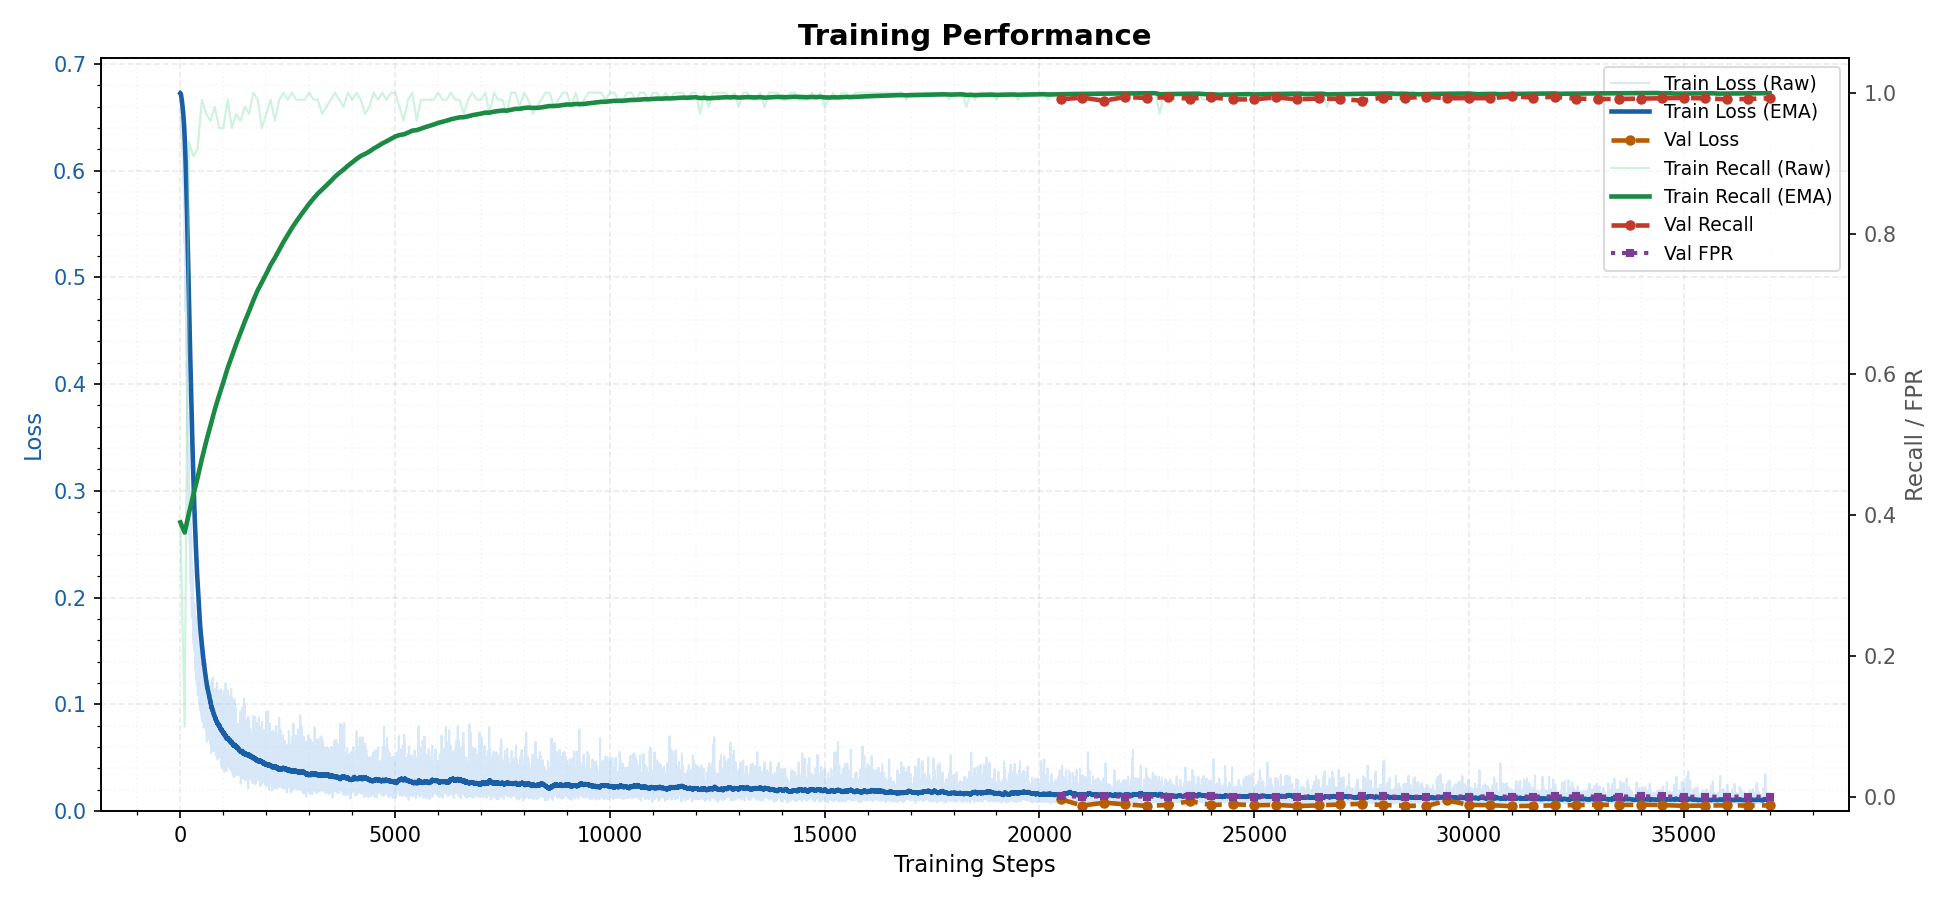
\includegraphics[width=\textwidth,height=0.4\textheight,keepaspectratio]{figures/ch05/training_performance_graph.png}
    \caption{Training Performance Metrics for the custom sanad.onnx Wake Word Model}
    \label{fig:wakeword_training}
\end{figure}

\section{Speech-to-Text (STT) Processing}
Transforming the raw audio of the user's voice into actionable text is handled differently depending on the network state, showcasing the system's hybrid flexibility.

\subsection{The Cloud Pathway (Multimodal Bypass)}
When operating online, the system entirely bypasses traditional STT transcription. Instead of converting speech to text first, the \texttt{llm\_node.py} intercepts the \texttt{audio://} path published by the wakeup node. It reads the raw audio bytes directly from the file system, packages them into a MIME audio object (\texttt{audio/wav}), and attaches it directly to the user's prompt. This payload is sent to Vertex AI's \texttt{gemini-2.5-flash} model, which natively understands audio data alongside text, reducing latency and transcription bottlenecks.

\subsection{The Local Pathway (Whisper \& Hallucination Filtering)}
In offline mode, the system relies on the \texttt{whisper\_node.py} to transcribe the audio into text.
\begin{itemize}
    \item \textbf{Execution:} It invokes a local installation of \texttt{whisper.cpp} (\texttt{whisper-cli}) via a system subprocess, feeding it the temporary WAV file and the optimized quantized model (\texttt{ggml-large-v3-q5\_0.bin}). It also passes the current active language flag (\texttt{-l}) to speed up inference.
    \item \textbf{Bulletproof Filtering:} A known issue with local Whisper models is "hallucination"—where the model invents text or hallucinates phantom subtitles when fed silence or background noise. To combat this, the node implements a strict filter. It drops any transcriptions that consist solely of punctuation and actively scans for a hardcoded list of garbage words (e.g., "Thanks for watching!", "Sous-titres", "شكرا للمشاهدة"). Only clean, validated text is published forward to the Commander node.
\end{itemize}

\section{Dynamic Context Management \& Prompt Engineering}
Before the LLM can make any decisions, it needs a complete, up-to-the-second understanding of the robot's environment and capabilities. This cognitive setup is the primary responsibility of the central orchestrator, \texttt{commander.py}.

\begin{figure}[htbp]
    \centering
    \resizebox{\textwidth}{!}{
    \begin{tikzpicture}[
        node distance=0.5cm and 1cm,
        file/.style={rectangle, draw=black!80, fill=gray!10, minimum height=0.6cm, align=center, font=\ttfamily\small},
        box/.style={rectangle, draw=black!80, fill=white, minimum height=0.8cm, align=center, font=\sffamily\small, rounded corners=2pt},
        arrow/.style={-{Stealth[scale=0.8]}, draw=black!80, thick}
        ]
        
        \node[file] (sys) {system\_prompt.yaml};
        \node[file, right=of sys] (lang) {current\_lang.yaml};
        \node[file, right=of lang] (rooms) {rooms.yaml};
        \node[file, right=of rooms] (state) {home\_state (dict)};
        \node[file, right=of state] (chat) {chat\_history (dict)};
        
        \node[box, below=2cm of rooms] (compiler) {Prompt Compiler \& String Interpolator};
        \node[box, below=1cm of compiler] (payload) {JSON Messages Payload};
        \node[box, below=1cm of payload] (call) {Service Call: /robot/llm\_query};
        
        \draw[arrow] (sys.south) -- ++(0,-0.5) -| (compiler.130);
        \draw[arrow] (lang.south) -- ++(0,-1.0) -| (compiler.110);
        \draw[arrow] (rooms.south) -- (compiler.north);
        \draw[arrow] (state.south) -- ++(0,-1.0) -| (compiler.70);
        \draw[arrow] (chat.south) -- ++(0,-0.5) -| (compiler.50);

        \draw[arrow] (compiler) -- (payload);
        \draw[arrow] (payload) -- (call);
    \end{tikzpicture}
    }
    \caption{Prompt Compilation and Context Injection Mapping}
    \label{fig:s6_context}
\end{figure}

The Commander does not just forward the user's query; it acts as a real-time context compiler, assembling a highly dynamic system prompt before querying the \texttt{/robot/llm\_query} service:

\begin{itemize}
    \item \textbf{Template Resolution:} It begins by loading a base prompt template from \texttt{system\_prompt.yaml}. It immediately replaces static placeholders with dynamic values, such as injecting the \texttt{\{LANGUAGE\_NAME\}} and pulling the current \texttt{\{ROOMS\_LIST\}} directly from the Nav2 \texttt{rooms.yaml} configuration file.
    \item \textbf{State Injection:} The Commander dynamically queries and serializes several critical state variables into JSON format, appending them to the bottom of the system prompt. This includes:
    \begin{itemize}
        \item \textbf{Device States:} The current ON/OFF status of the AC, heater, lights, and TV (\texttt{self.home\_state}).
        \item \textbf{Communication Context:} The names of available Telegram contacts loaded from \texttt{telegram\_contacts.yaml}.
        \item \textbf{Unread Notifications:} Any pending messages waiting in the \texttt{telegram\_messages.yaml} inbox.
    \end{itemize}
    \item \textbf{Conversational Memory (Rolling Window):} To allow for natural, multi-turn conversations (e.g., "Turn on the light," followed by "Actually, turn it off"), the Commander maintains a rolling chat history. It stores the role and content of the last 10 interactions.
\end{itemize}

Finally, the Commander bundles the heavily engineered system prompt together with the rolling chat history and the user's latest command into a single, comprehensive JSON payload, which is then dispatched to the LLM for evaluation.

\section{LLM Reasoning \& Intent Parsing}
Once the LLM (whether cloud-based Gemini or local Qwen) processes the highly contextual system prompt and user command, it must return a response that the robotic system can programmatically understand. It does this by outputting a strictly formatted JSON payload alongside its conversational text.

When the \texttt{llm\_node} returns the AI's response back to the \texttt{commander.py} node, the system runs an extraction routine. The \texttt{extract\_json} method uses regular expressions to strip out extraneous text or reasoning tokens (such as \textless \texttt{think} \textgreater \ tags common in local models) and isolates the core JSON dictionary.

This JSON payload is parsed to determine the user's core intent. The model categorizes the request by generating specific keys such as \texttt{intent}, \texttt{target}, \texttt{action}, \texttt{navigate\_to}, or simply a \texttt{response} string. By inspecting these keys, the system inherently knows whether it needs to control hardware, move to a new location, interact with external APIs, or simply chat with the user.

\section{The Intent Router \& Action Execution}

\begin{figure}[htbp]
    \centering
    \resizebox{\textwidth}{!}{
    \begin{tikzpicture}[
        node distance=0.8cm and 0.5cm,
        box/.style={rectangle, draw=black!80, fill=white, minimum height=0.8cm, minimum width=2.8cm, align=center, font=\sffamily\small, rounded corners=2pt},
        decision/.style={diamond, aspect=2, draw=black!80, align=center, font=\sffamily\small, rounded corners=1pt},
        arrow/.style={-{Stealth[scale=0.8]}, draw=black!80, thick}
        ]
        
        \node[box] (res) {LLM Response};
        \node[decision, below=of res] (parser) {Intent Parser};
        
        \node[box, below left=1.5cm and 2.5cm of parser] (nav) {Navigation Logic};
        \node[box, left=0.5cm of nav] (sm) {Smart Home Logic};
        
        \node[box, below right=1.5cm and 2.5cm of parser] (tg) {Telegram Logic};
        \node[box, right=0.5cm of tg] (conv) {Conversational Bypass};

        \draw[arrow] (res) -- (parser);
        
        \draw[arrow] (parser.south) -- ++(0,-0.5) -| node[pos=0.25, above, font=\sffamily\scriptsize] {control} (sm.north);
        \draw[arrow] (parser.south) -- ++(0,-0.5) -| node[pos=0.25, above, font=\sffamily\scriptsize] {navigate} (nav.north);
        \draw[arrow] (parser.south) -- ++(0,-0.5) -| node[pos=0.25, above, font=\sffamily\scriptsize] {telegram} (tg.north);
        \draw[arrow] (parser.south) -- ++(0,-0.5) -| node[pos=0.25, above, font=\sffamily\scriptsize] {response} (conv.north);

        \node[box, below=of sm] (pubsm) {Pub: /robot/smarthome};
        \node[box, below=of nav] (pubnav) {Pub: /robot/nav\_command};
        \node[box, below=of tg] (pubtg) {Pub: /robot/telegram};
        \node[box, below=of conv] (pubtts) {Pub: /robot/speak};

        \draw[arrow] (sm) -- (pubsm);
        \draw[arrow] (nav) -- (pubnav);
        \draw[arrow] (tg) -- (pubtg);
        \draw[arrow] (conv) -- (pubtts);
    \end{tikzpicture}
    }
    \caption{ROS 2 Intent Demultiplexer and Topic Routing}
    \label{fig:s8_router}
\end{figure}

The \texttt{commander.py} node serves as the central switchboard, taking the parsed JSON dictionary and distributing the commands to the appropriate ROS 2 subsystems.

\subsection{Smart Home Control}
If the JSON dictionary contains an \texttt{intent} labeled \texttt{control} or a dedicated \texttt{controls} list, the router targets the IoT devices.
\begin{itemize}
    \item It extracts the \texttt{target} (e.g., "ac", "light", "tv") and the desired \texttt{action} (e.g., "on", "off").
    \item Before commanding the hardware, the Commander updates its internal \texttt{self.home\_state} dictionary to reflect the new status (e.g., changing the AC state to 'on'). This ensures the LLM knows the device is already on during the next conversation turn.
    \item Finally, the routing logic publishes the control array as a JSON string to the \texttt{/robot/smarthome\_command} topic for the hardware actuators to execute.
\end{itemize}

\subsection{Autonomous Navigation}
When the user asks the robot to move, the LLM includes a \texttt{navigate\_to} key in its JSON output.
\begin{itemize}
    \item The Commander dynamically reloads the system's spatial coordinates from the \texttt{rooms.yaml} file to ensure it has the most up-to-date map data.
    \item It matches the requested room name to its precise X, Y, and Z pose coordinates.
    \item The router then publishes the movement intent to the \texttt{/robot/nav\_command} topic. Simultaneously, it initiates an asynchronous service call to the \texttt{rooms/navigate} Nav2 endpoint, which physically commands the robot's drive base to travel to the destination.
\end{itemize}

\subsection{Asynchronous Communication (Telegram)}
The Commander can seamlessly interface with external messaging services by parsing specific Telegram intents.
\begin{itemize}
    \item \textbf{Sending Messages:} If the intent is \texttt{telegram}, the system extracts the \texttt{contact} name and the \texttt{message} text. It verifies the contact against the dynamically loaded \texttt{telegram\_contacts.yaml} database. If a match is found, it publishes the payload to the \texttt{/robot/telegram/send} topic, where the dedicated \texttt{telegram\_node.py} handles the API web request.
    \item \textbf{Reading/Clearing Notifications:} If the intent is \texttt{read\_telegram}, the Commander determines the scope (either clearing all messages or just messages from a specific sender) and publishes a clear command to the \texttt{/robot/telegram/clear} topic, which updates the local inbox file.
\end{itemize}

\subsection{The Conversational Bypass}
Not every user interaction requires a physical action. If the user asks a general knowledge question ("How do car gears work?") or requests a recipe, the LLM will generate a JSON payload lacking movement or control intents, featuring only the \texttt{response} key.
\begin{itemize}
    \item The Commander extracts this \texttt{response} string.
    \item It completely bypasses all the hardware action routers and publishes the text directly to the \texttt{/robot/speak} topic.
    \item This triggers the TTS node to vocalize the response, creating a seamless conversational experience where the robot acts as a pure knowledge assistant in the user's spoken language.
\end{itemize}

\section{Text-to-Speech (TTS) Synthesis}
The final stage of the Sanad voice pipeline is the \texttt{tts\_node.py}, which is responsible for giving the robot a voice. It constantly listens to the \texttt{/robot/speak} topic for text payloads dispatched by the Commander node. To ensure the robot's voice is responsive and natural, the node implements two distinct playback strategies depending on the network availability.

\begin{figure}[htbp]
    \centering
    \begin{tikzpicture}[
        node distance=0.8cm and 2cm,
        box/.style={rectangle, draw=black!80, fill=white, minimum height=0.6cm, minimum width=3cm, align=center, font=\sffamily\small, rounded corners=2pt},
        decision/.style={diamond, aspect=2, draw=black!80, align=center, font=\sffamily\small, rounded corners=1pt},
        arrow/.style={-{Stealth[scale=0.8]}, draw=black!80, thick},
        dashedarrow/.style={-{Stealth[scale=0.8]}, draw=black!80, thick, dashed}
        ]
        
        \node[box] (sub) {Sub: /robot/speak};
        \node[box, below=of sub] (stop) {Trigger Stop Event};
        \node[decision, below=of stop] (cloud) {use\_cloud?};
        
        \node[box, below left=1cm and 0.2cm of cloud] (stream) {Stream Audio Chunks\\(Vertex AI)};
        \node[box, below right=1cm and 0.2cm of cloud] (piper) {Subprocess Piper TTS};
        
        \node[box, below=of stream] (q) {Thread-Safe\\Audio Queue};
        \node[box, below=of piper] (wav) {Save /tmp/robot\_speech.wav};

        \node[box, below=3.5cm of cloud] (spk) {Robot Speakers};

        \draw[arrow] (sub) -- (stop);
        \draw[arrow] (stop) -- (cloud);
        
        \draw[arrow] (cloud.west) -| node[above, near start, font=\sffamily\scriptsize] {True} (stream.north);
        \draw[dashedarrow] (cloud.east) -| node[above, near start, font=\sffamily\scriptsize] {False} (piper.north);
        
        \draw[arrow] (stream) -- (q);
        \draw[dashedarrow] (piper) -- (wav);
        
        \draw[arrow] (q.south) |- (spk.west);
        \draw[dashedarrow] (wav.south) |- (spk.east);
    \end{tikzpicture}
    \caption{Hybrid Text-to-Speech Synthesis and Audio Buffering}
    \label{fig:s9_tts}
\end{figure}

\subsection{The Cloud Pathway (Real-Time Streaming)}
When the system operates online, it connects to Google Cloud's Vertex AI using the \texttt{gemini-2.5-flash-preview-tts} model.
\begin{itemize}
    \item To drastically reduce latency, the system employs a streaming architecture rather than waiting for the entire response to be synthesized.
    \item The node's \texttt{AudioPlayer} class opens a continuous \texttt{sounddevice} output stream in a background thread.
    \item As the cloud API returns individual audio chunks, the system intercepts the raw PCM bytes, dynamically resamples them via linear interpolation (from the input rate of 24,000 Hz to the system output rate of 44,100 Hz), and pushes them into a playback queue.
    \item This allows the robot to begin speaking the first words of a sentence while the rest of the paragraph is still being generated on the server.
\end{itemize}

\subsection{The Local Pathway (Offline Synthesis)}
In offline mode, the node gracefully falls back to a local Piper TTS engine.
\begin{itemize}
    \item It executes a subprocess that calls the \texttt{piper} binary, feeding it the text alongside a local ONNX voice model (such as \texttt{ar\_JO-kareem-medium.onnx}).
    \item Unlike the cloud's chunked streaming, the local Piper execution generates a complete, temporary WAV file (\texttt{/tmp/robot\_speech.wav}).
    \item Once the synthesis is finished, the \texttt{AudioPlayer} reads the file using the \texttt{soundfile} library and plays it synchronously through the speakers.
\end{itemize}

\subsection{Interrupt \& Audio Management}
Regardless of whether the TTS is streaming from the cloud or playing a local WAV file, the node features robust audio thread management. The \texttt{AudioPlayer} class utilizes threading events (\texttt{stop\_event}) to track the playback state. If the robot is in the middle of speaking a long paragraph and the user issues a new command, the TTS node will instantly trigger the stop event, close the audio stream, drain the playback queue, and prepare to speak the newly generated response.

\section{Summary and Transition}
This chapter has detailed the hybrid voice control interface, explaining how spoken Arabic commands are parsed into system goals. The next chapter, Chapter 6 (Server Architecture and Design), describes the Node.js integration server that bridges these external client interfaces with the core ROS 2 message system.